This tutorial is based on the
\href{http://www.wheat-expression.com/}{\lstinline!Wheat Expression Browser!}.
However, the principles are the same for any transcriptome study which
is powered by the expVIP graphical interface.

\section{\textbf{Home Page}}\label{home-page}

The home page allows the user to insert a gene name to search and to
define which studies are to be included in the visualisation interface.
By default all studies are selected, but users can select/deselect a
study by simply clicking on the specific button.

You can also compare expression between two genes by introducing both
gene names in the boxes and pressing the \lstinline!Compare! button.

Alternatively you can compare expression across multiple genes (up to
50) to generate a heatmap. You can add a list of genes separate by
commas or one gene per line in the \lstinline!Multiple genes! box.

All gene names are based on the transcriptome reference used for expVIP:
for the case of the Wheat Expression Browser we used the IWGSC
transcriptome available through
\href{http://plants.ensembl.org/Triticum_aestivum/Info/Annotation/\#genebuild}{Ensembl
Plants} release 26.

\section{\textbf{Visualisation
interface}}\label{visualisation-interface}

\subsection{\textbf{Single gene or two-gene
comparison}}\label{single-gene-or-two-gene-comparison}

Once the gene expression loads the page includes several features. These
are shown below and explained point by point:

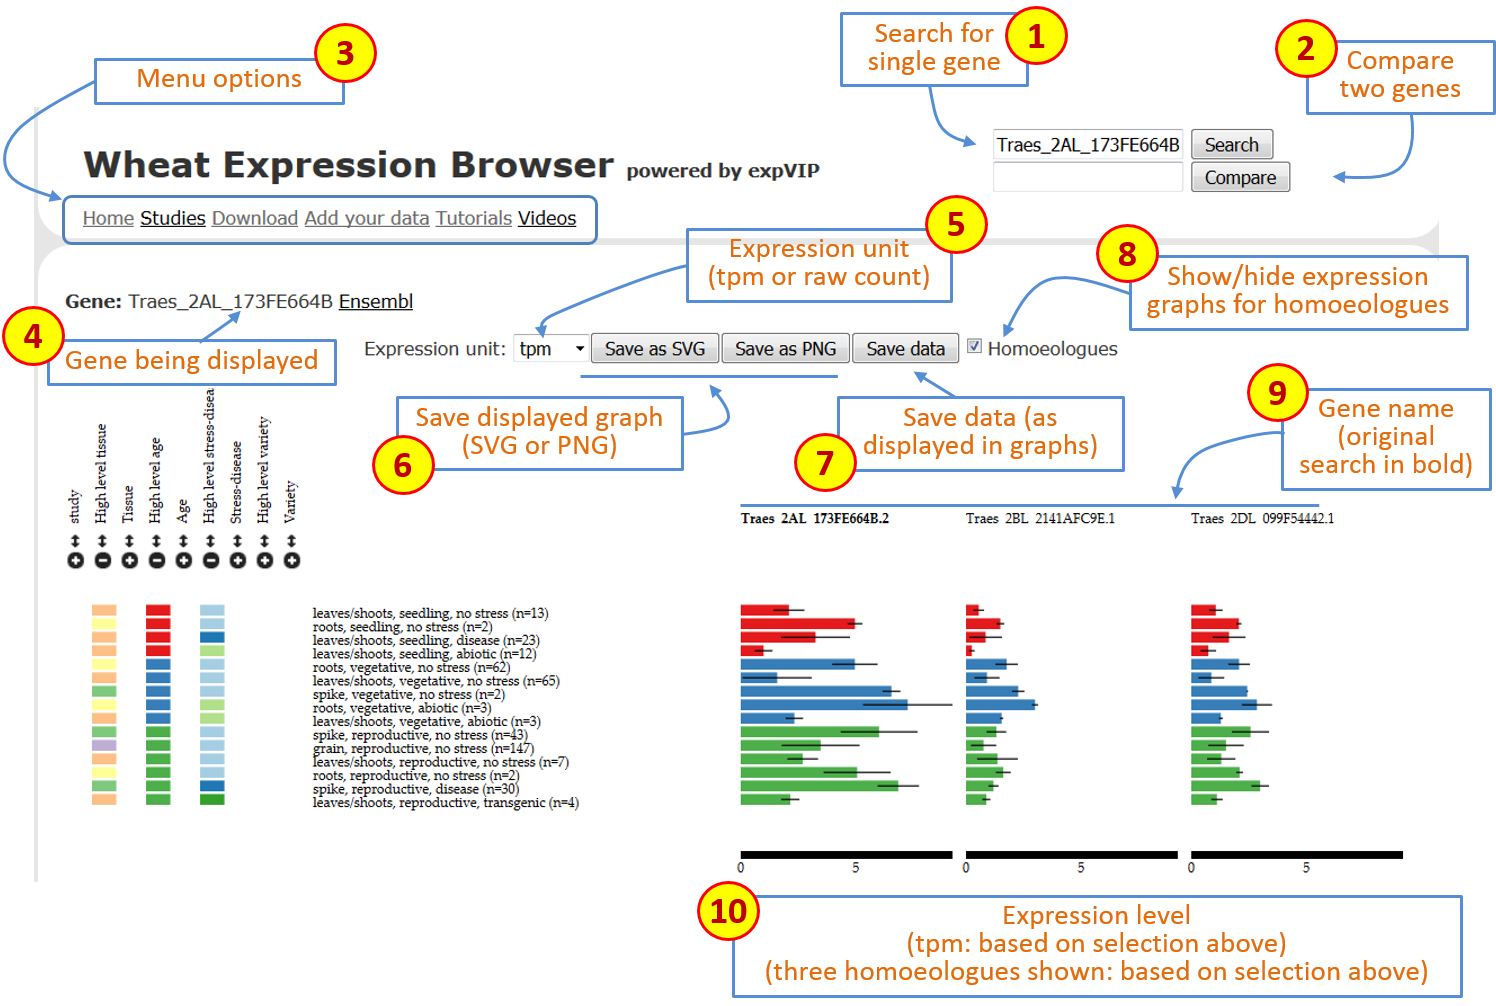
\includegraphics{images/Figure1.png} \textbf{Figure 1:} Overall
description of features on Wheat Expression Browser

\begin{enumerate}
\def\labelenumi{\arabic{enumi}.}
\itemsep1pt\parskip0pt\parsep0pt
\item
  \textbf{\lstinline!Search box!}: at any point you can type or copy a
  new gene name (based on Ensembl Plants nomenclature) and generate a
  new set of expression data.
\item
  \textbf{\lstinline!Compare box!}: you can type a second gene name and
  press the \lstinline!Compare! button to generate two expression graphs
  drawn at the same scale.
\item
  \textbf{\lstinline!Menu options!}: this includes a series of links to
  different options:\\
\end{enumerate}

\begin{itemize}
\itemsep1pt\parskip0pt\parsep0pt
\item
  \textbf{\lstinline!Home!}: return to \lstinline!home! screen.
\item
  \textbf{\lstinline!Studies!}: opens up a popup screen with a summary
  and short description of each study and a link to manuscript.
\item
  \textbf{\lstinline!Download!}: link to download all the wheat
  expression database including \lstinline!tpm! and \lstinline!counts!
  and associated metadata.
\item
  \textbf{\lstinline!Add your data!}: link to GitHub to download virtual
  machine.
\item
  \textbf{\lstinline!Tutorials!}: link to Wheat Expression Browser
  Tutorial.
\item
  \textbf{\lstinline!Videos!}: link to Wheat Expression Browser Video
  Tutorial.
\end{itemize}

\begin{enumerate}
\def\labelenumi{\arabic{enumi}.}
\item
  \textbf{\lstinline!Gene!}: shows the gene which is currently being
  displayed with link to Ensembl Plants gene page.
\item
  \textbf{\lstinline!Expression unit!}: allows user to select the
  expression unit used to visualise the expression data. This can be
  either ``transcript per million (\lstinline!tpm!)'' or ``estimated
  counts (\lstinline!counts!)''. We have not provided RPKM given the
  inconsistencies generated across samples when using this measure. A
  detailed discussion can be found in
  \href{http://www.ncbi.nlm.nih.gov/pubmed/22872506}{Wagner \emph{et
  al}} (2012). It is important to mention that \lstinline!tpm! is
  preferred over RPKM since it allows an easier comparison for
  abundances between samples. However it is important to stress that
  while \lstinline!tpm! serves as a relative measure to compare genes
  across experiments, a proper normalisation and statistical analysis
  with differential gene expression programs must be performed.
  \lstinline!expVIP! generates outputs which allow easy implementation
  of \lstinline!sleuth!, \lstinline!DESeq! and \lstinline!EdgeR!.
\item
  \textbf{\lstinline!Save graph!}: these two buttons allow users to save
  the current graphs in either \lstinline!SVG! (to work on Adobe
  Ilustrator) or as \lstinline!PNG! files. The graphical file will
  render based on the current selection and order of factors as
  displayed on the screen.
\item
  \textbf{\lstinline!Save data!}: this allows the user to download a
  \lstinline!csv! file with the data based on the current selection and
  order of factors as displayed on the screen. The data will include the
  standard errors and the number of samples that make up each value.
\item
  \textbf{\lstinline!Homoeologues!}: by clicking on this button, the
  \lstinline!Wheat Expression Browser! will display the expression
  graphs of known homoeologues of the original primary gene. This gene
  name will remain in bold and the homoeologous graphs will be displayed
  according to A, B, D genome ordering. When homoeologues are displayed
  the same expression scale is used across graphs and the sorting and
  filtering of factors is simultaneous to allow easier comparison.
\item
  \textbf{\lstinline!Gene names!}: gene name for corresponding graph.
  When homoeologues are shown the original gene used for the search is
  shown in bold.
\item
  \textbf{\lstinline!Expression level!}: the expression level adjusts
  according to the expression of each set of gene homoeologues. The
  scale remains consistent across homoeologues to allow easier
  comparison. The values are based on the unit selected in the
  \lstinline!expression unit! box (see point 5 above).
  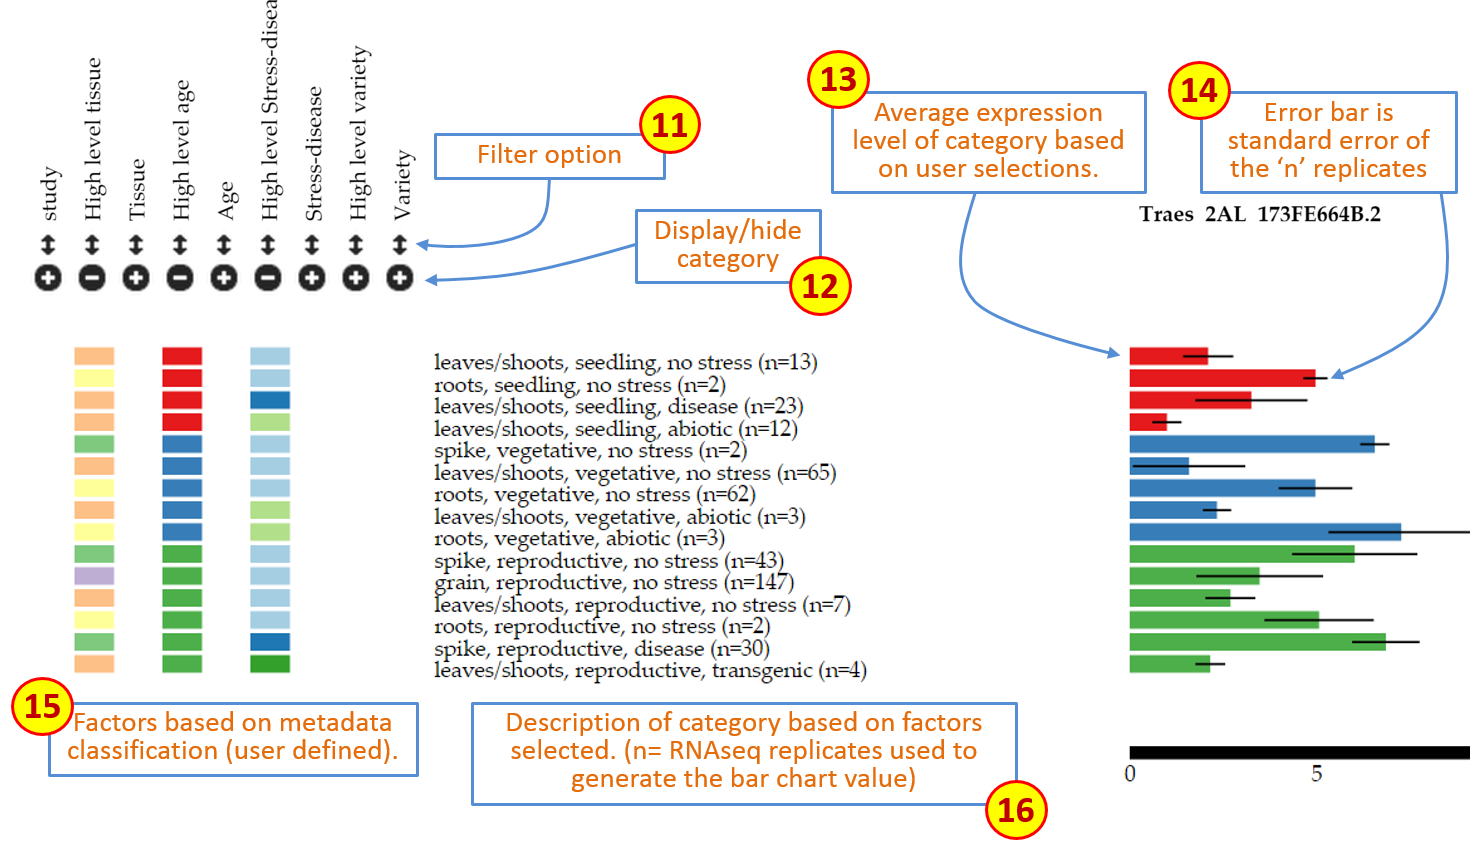
\includegraphics{images/Figure2.png} \textbf{Figure 2:} Overall
  description of features on Wheat Expression Browser (continued)
\item
  \textbf{\lstinline!Filter!}: This feature open a pop-up window which
  reveals all the levels within the particular category. All levels are
  pre-selected, but users can choose to display specific levels by
  selecting or deselecting them accordingly. If a level is deselected,
  then the data associated with this factor is removed from the graph.
  Within the pop-up window levels can also be re-arranged according to
  the user's preference by dragging the level to the specific position
  within the pop-up window (see Features section below).
\item
  \textbf{\lstinline!Display/hide category!}: Each individual category
  can be displayed or hidden by pressing the \lstinline!+/-! button.
  When a category is displayed, the expression graphs will re-arrange
  according to the new category which has been introduced. If a category
  is hidden, then the graphs will also adjust accordingly. Data is not
  removed when doing this, rather it is grouped within the categories
  selected such that the total samples displayed remains the same. The
  colours within the category correspond to unique values or levels (up
  to 24 different colours) and are also used in the bar graphs
  corresponding to the expression data.\\
\item
  \textbf{\lstinline!Expression bars!}: These bars represent the
  expression level of the ``n'' samples which are grouped according to
  the factors chosen based on the selection criteria (11 and 12 above).
  When hovering over the bar with the mouse a small tooltip will
  indicate the expression level (\lstinline!tpm! or \lstinline!counts!)
  and the standard error (sem) used for the error bars (see 14)
\item
  \textbf{\lstinline!Error bars!}: Standard error of the means for the
  ``n'' expression values on which the bar graph is based.
\item
  \textbf{\lstinline!Factors!}: Coloured rectangles represent the
  categories which are displayed according to the factors chosen based
  on the selection criteria (11 and 12 above). When hovering above the
  rectangles a tooltip will appear to show the long name of the level
  being examined.
\item
  \textbf{\lstinline!Description!}: Text description of the factors
  chosen based on the selection criteria (11 and 12 above) and the
  number of RNAseq samples (n) which meet this specific criterion.

  \subsection{\textbf{Multiple gene
  comparisons}}\label{multiple-gene-comparisons}
\item
  \textbf{\lstinline!Expression unit!}: For heatmaps, log2(tpm) is
  suggested as the expression unit as this provides better resolution to
  compare multiple genes across several categories.
\item
  \textbf{\lstinline!Heatmap!}: Expression data is represented as a
  heatmap. As for single genes, categories can be sorted and filtered
  using the same tools. Gene names appear on the top of each column.
  Currently, up to 50 genes can be visualised in one heatmap. In Figure
  3, for example, the two right-most genes are expressed solely in
  grains, with one being expressed to higher levels as suggested by the
  dark blue colour.
\item
  \textbf{\lstinline!Scale!}: Colour scale for the expression values in
  the heatmap. The values adjust according to the highest tpm value
  being displayed within the current heatmap visualisation. Since tpm
  values below 2 are considered as very low expressed genes and log2
  values of tpm\textless{}1 result in negative expression values, we
  forced tpm values below 1 to have a log2 value of cero
  (i.e.~log2(\textless{}1)=0).
\end{enumerate}

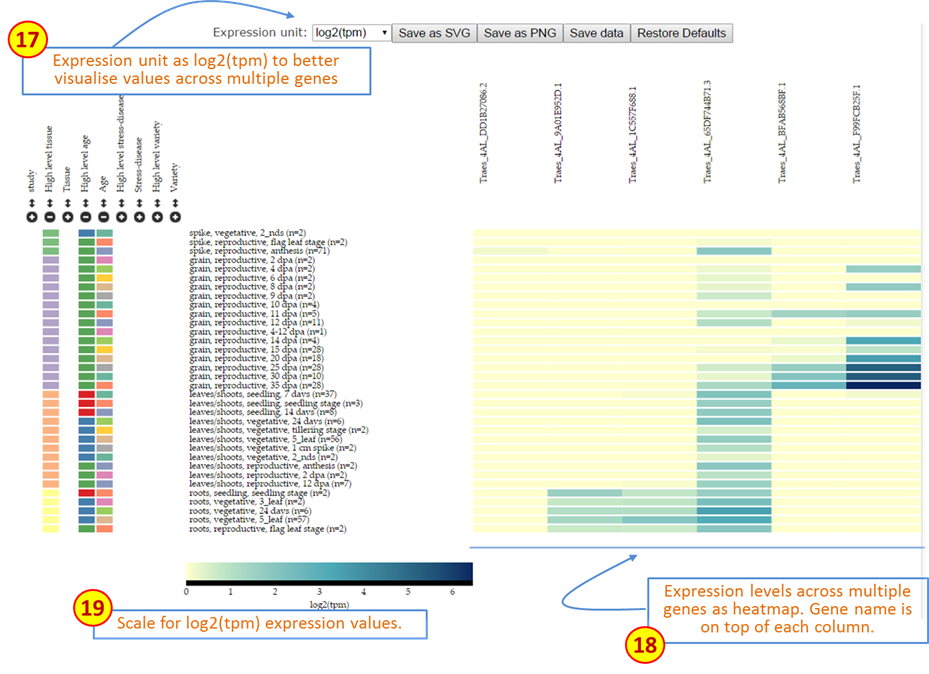
\includegraphics{images/Figure2a.png} \textbf{Figure 3:} Description of
features on Wheat Expression Browser using Multiple gene comparisons.

\subsection{\textbf{Features}}\label{features}

\subsubsection{\textbf{Sorting}}\label{sorting}

Factors can be sorted within each category in two ways.

\begin{enumerate}
\def\labelenumi{\arabic{enumi}.}
\itemsep1pt\parskip0pt\parsep0pt
\item
  The first is by simply clicking the mouse on top of the coloured
  rectangles underneath the heading. For example in Figure 2 samples are
  sorted on \lstinline!High level age! from \lstinline!seedling! (red),
  \lstinline!vegetative! (blue) to \lstinline!reproductive! (green). If
  the user clicks on any of the coloured rectangles in the
  \lstinline!High level tissue! category, then the graph is
  automatically reorganised based on this factor. In this case it
  includes four categories as defined by the user in the metadata and
  the bar graphs on the right hand side change colour according to the
  latest factor used for sorting. The previous factor used (in this case
  \lstinline!high level age!) remains as a secondary sorting factor
  (Figure 3). 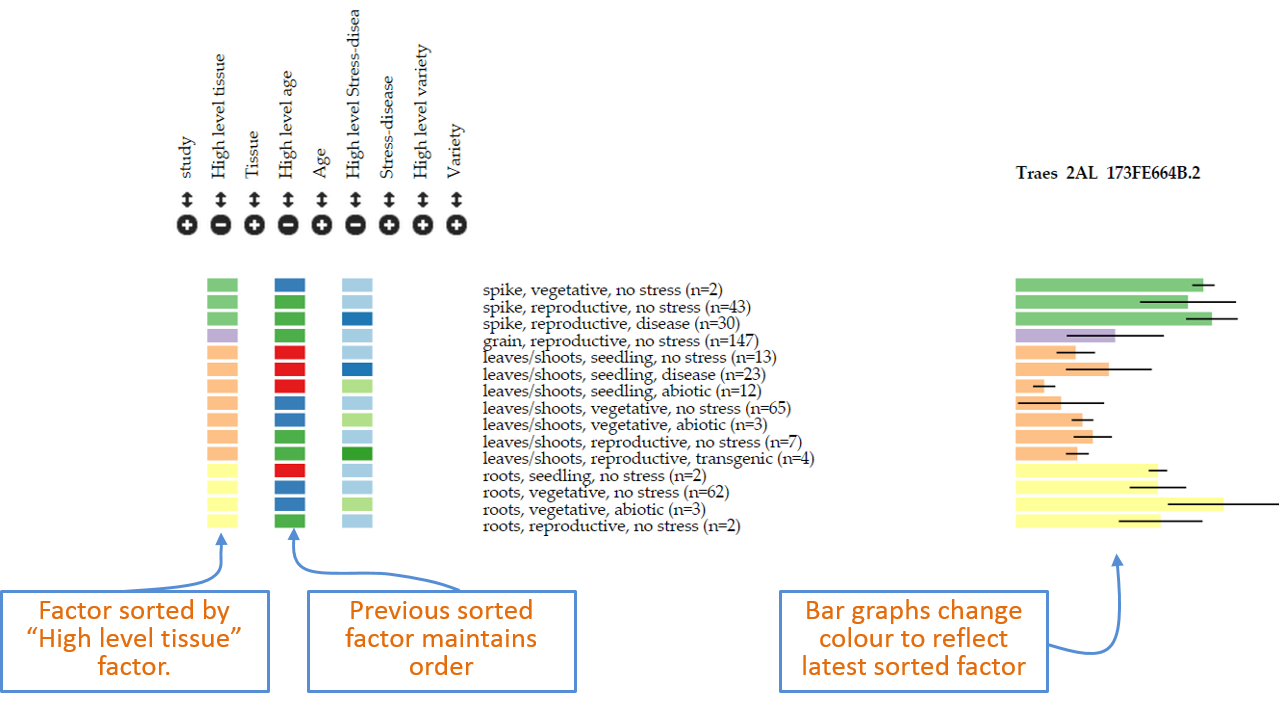
\includegraphics{images/Figure3.png} \textbf{Figure 4:}
  Example of new sorting of data based on clicking of rectangles within
  ``high level tissue''.
\item
  Alternatively, the user can define the exact order of factors within
  the browser interface. To do so the \lstinline!filter! option (point
  11 above) can be used. By clicking on the double arrow button the user
  opens a pop-up window which shows the levels within the factor. In
  this example by pressing the double-arrow underneath
  \lstinline!high level tissue! a pop-up with four levels appears based
  on the order as determined in the user defined metadata
  (\lstinline!spike!, \lstinline!grain!, \lstinline!leaves/shoots!,
  \lstinline!roots!). To rearrange this, the user can simply click, hold
  and drag the level to the desired position. This will automatically
  re-arrange the data based on the new order and the corresponding graph
  and legends will follow suit. The bottom panel of Figure 5 shows a new
  order of \lstinline!roots!, \lstinline!leaves/shoots!,
  \lstinline!spike! and \lstinline!grain!.
  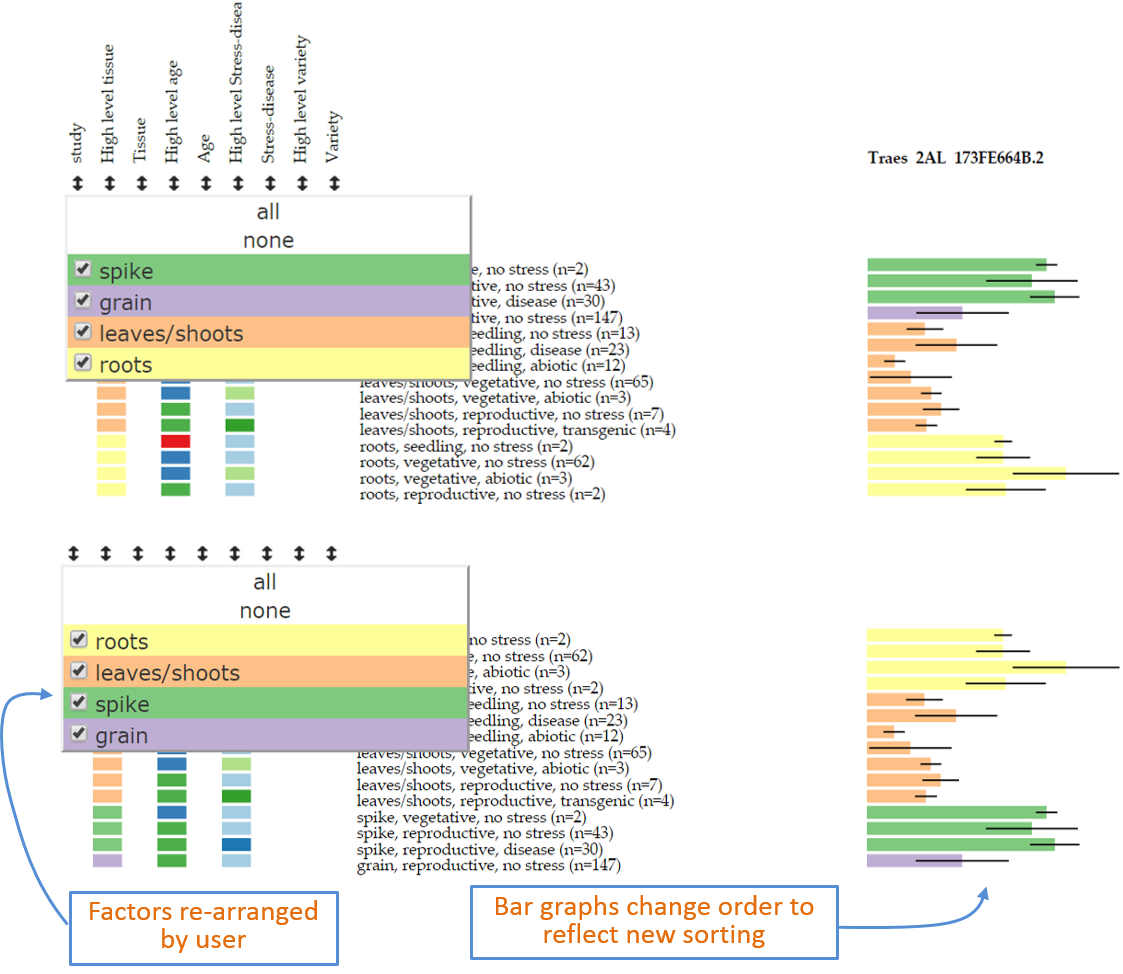
\includegraphics{images/Figure4.png} \textbf{Figure 5:} Example of
  sorting of data based on new user defined order within the filter
  pop-up window.
\end{enumerate}

\subsubsection{\textbf{Filtering}}\label{filtering}

In cases it may be required to remove certain samples from the
visualisation. Note that displaying or hiding a category (point 12
above) does not remove the underlying data from the visualisation: this
just simply groups the data within the selected category. Therefore to
remove samples from the visualisation the user can open the filter
pop-up as described for the \lstinline!Sorting! option. Individual
levels within the category can then be removed by using the
``check-box'' on the left hand side of the level name. By de-selecting a
given level (in the example for Figure 6 we have deselected
\lstinline!leaves/shoots! and \lstinline!spike!), samples defined as
such will be removed from the analysis and will not be shown in the bar
graphs. In Figure 6 now only two levels remain (\lstinline!roots! and
\lstinline!grains!) and hence the bar graphs only show these two levels.
Notice that the numbers of samples which comprise each bar graph are the
same as those on Figure 5. The pop-up window also includes an
\lstinline!all! and \lstinline!none! option to rapidly select/deselect
individual samples. The filtering option can be used on any factor: for
example to remove a complete study from the analysis the easiest way is
to select the \lstinline!study! filtering pop-up on the far left and
deselect the study in question.

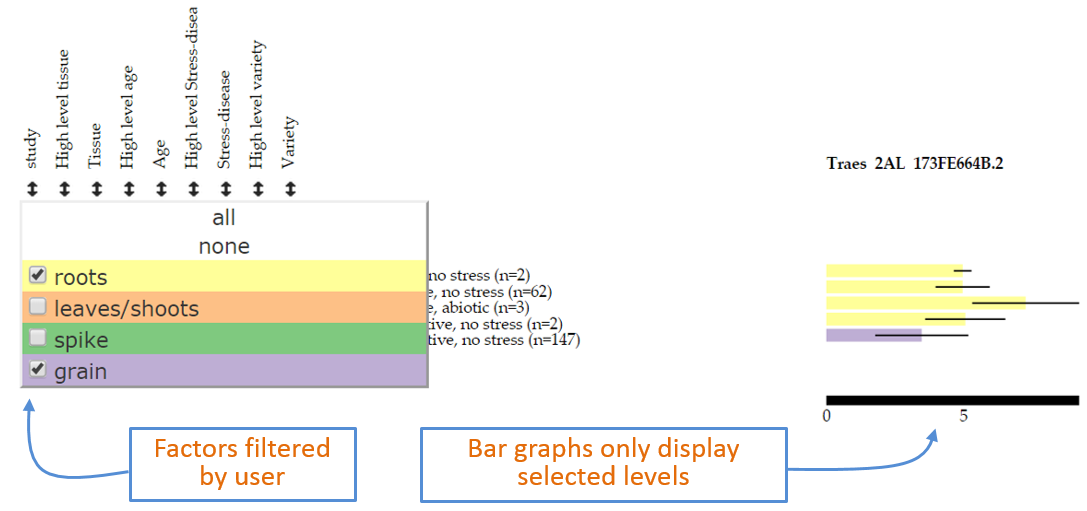
\includegraphics{images/Figure5.png} \textbf{Figure 6:} Example of
filtering data based on user defined selection within the filter pop-up
window.
